\documentclass[report.tex]{subfiles}

\begin{document}

\section*{\centering Introduction}

Electronics sports, hereafter will be referred to as esports, are a form of competition using electronic systems, in particular video games, controlled by human players. In recent years, the revenue and audience have seen a rapid growth with an estimation of over 300 million viewers in 2016 and over \$450 million in global revenue, and it is expected to see a formidable growth in the near future.\footnote{https://newzoo.com/insights/articles/esports-revenues-will-reach-696-million-in-2017/}

The esports industry utilizes many different platforms such as personal computers (PCs), X-Box, Playstation, and since everything is electronic we could potentially utilize all that data that is being generated for various kinds of analyses. That could help organizations/teams find better strategies, improve the viewer experience, and help newcomers getting accustomed to the different games in a short time span, thus further increase the growth.

\subsection*{DOTA 2}

Defense of the Ancients (DOTA 2) is a so called multiplayer online battle arena (MOBA) video game developed by Valve Corporation made first available in 2011. The game plays out as two teams of 5 players battle against each other where each player controls a hero, a character with unique abilities. The aim is to destroy the opponents ancient and thus win the game. How that is achieved varies from game to game, from fast paced game that are under 20 minutes to long drawn out game lasting over 60 minutes.

\subsubsection*{Draft Phase}

The draft phase is the time the two teams pick their heroes, as of \today, there are 113 unique heroes to select from, that will be played during the gameplay phase. Each team has to pick 5 heroes, ban 5 heroes, and banned heroes are unavailable for either team to pick. The actual order is shown in figure \ref{fig:picks_bans}.

\begin{figure}[H]
  \centering
  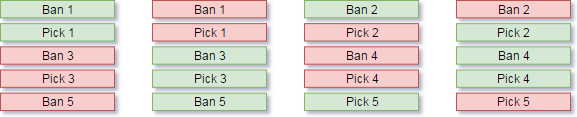
\includegraphics[width=\textwidth]{./images/dota2}
  \caption{The pick and ban orders read from left to right, top to bottom. The colors represent the two teams.}
   \label{fig:picks_bans}
\end{figure}

This phase is very tactical and determines a lot how the gameplay will pan out. The reason for that is that heroes have their strengths and weaknesses. The heroes of a team composition fulfill different purposes, very broadly speaking at what time periods they are weak or powerful. A useful term is the \textit{metagame} that is globally influential on what heroes are being picked. It describes what strategies, heroes, and ideas about the game is currently popular and is heavily influenced by the developers' changes to the game, but also as the professional community figures out what works well.

\subsection*{Questions}

In this report I am going to use cluster and association analysis in order to figure out if it is possible to find relevant patterns that could help newcomers to watching professional DOTA 2. The questions I have set to explore are mainly based the relationships between heroes. The relationship is either \textit{synergistic}, e.g., hero X works well with hero Y, or \textit{counteractive}, e.g., hero X is strong against hero Y.

\begin{itemize}
\item When should I pick hero X?
\item Which heroes should I pick along with hero X?
\item What are common team compositions overall?
\item Do team compositions change between tournaments?
\end{itemize}

\end{document}
